% Asset ID: A22StatisticalHypothesisTestingTikZ-003
% Source: Chapter 7 Hypothesis Testing Binomial transcript
% Related lesson section: Critical regions
% Purpose: Show one-tailed critical regions.
% Related LO IDs: A22-HT-LO001, A22-HT-LO002, A22-HT-LO003

\documentclass[tikz,border=8pt]{standalone}
\usepackage{amsmath}
\usetikzlibrary{arrows.meta, positioning, decorations.pathreplacing}
\begin{document}
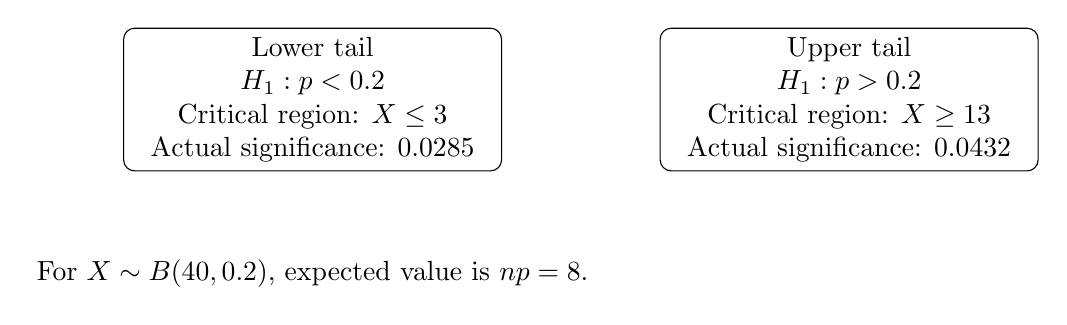
\begin{tikzpicture}[node distance=1.2cm, box/.style={draw, rounded corners, align=center, minimum width=4.8cm, minimum height=1.0cm}, arrow/.style={-{Latex[length=3mm]}, thick}]

\node[box] (left) {Lower tail\\\(H_1:p<0.2\)\\Critical region: \(X\leq 3\)\\Actual significance: \(0.0285\)};
\node[box, right=2cm of left] (right) {Upper tail\\\(H_1:p>0.2\)\\Critical region: \(X\geq 13\)\\Actual significance: \(0.0432\)};
\node[below=1cm of left, align=center] {For \(X\sim B(40,0.2)\), expected value is \(np=8\).};

\end{tikzpicture}
\end{document}
